
%#########################12########################
\stepcounter{section}
\begin{center}
	\textbf{\color{color2}\LARGE \thesection} \quad  \textbf{\LARGE Morbilidad relacionada} \addcontentsline{toc}{section}{\numberline{\thesection} Morbilidad relacionada}
\end{center}
$\ $ \\[-2.3cm]
\cajita{%
	Diarrea}%
{%
	Los casos de diarrea han ido en aumento desde el año 2011, reportándose un total de 331,874 para el 2015.
}%
{%
	Niños menores de cinco años que recibieron atención médica por diarrea} %
{%
	República de Guatemala, serie histórica, número de niños} %
{%
	\begin{tikzpicture}[x=1pt,y=1pt]  \input{graficas/5_12.tex}  \end{tikzpicture}}%
{%
	Sigsa} %


%#########################13########################

\cajita{%
	Diarrea según sexo}%
{%
	Los casos de diarrea para el 2015 se presentaron en cantidades similares en niños y niñas, teniendo menor ocurrencia en las niñas. 
	}%
{%
	Niños menores de cinco años que recibieron atención médica por diarrea, según sexo} %
{%
	República de Guatemala, 2015, número de niños} %
{%
	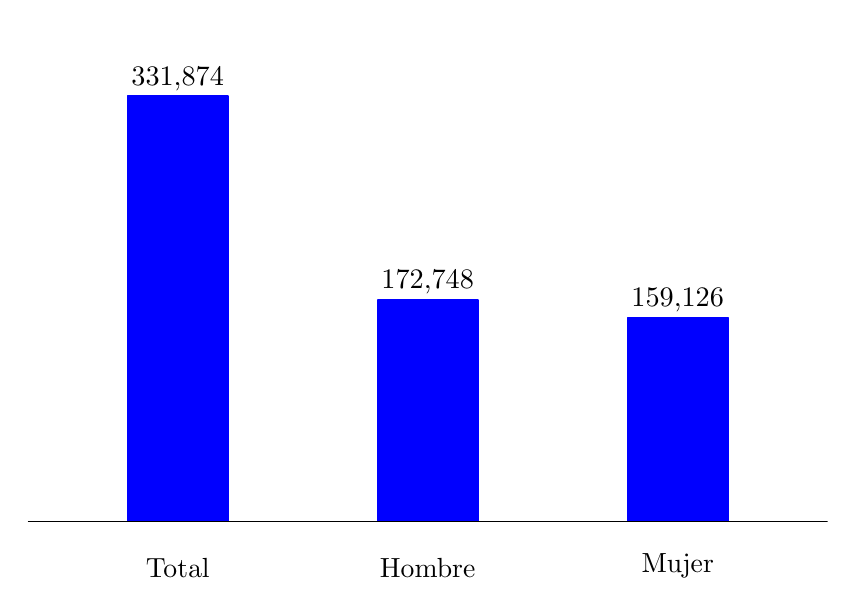
\begin{tikzpicture}[x=1pt,y=1pt]  % Created by tikzDevice version 0.9 on 2016-03-03 05:26:37
% !TEX encoding = UTF-8 Unicode
\definecolor{fillColor}{RGB}{255,255,255}
\path[use as bounding box,fill=fillColor,fill opacity=0.00] (0,0) rectangle (289.08,198.74);
\begin{scope}
\path[clip] (  0.00,  0.00) rectangle (289.08,198.74);

\path[] (  0.00,  0.00) rectangle (289.08,198.74);
\end{scope}
\begin{scope}
\path[clip] (  0.00,  0.00) rectangle (289.08,198.74);

\path[] (  0.00, 12.77) rectangle (289.08,181.67);

\path[] ( 54.20, 12.77) --
	( 54.20,181.67);

\path[] (144.54, 12.77) --
	(144.54,181.67);

\path[] (234.88, 12.77) --
	(234.88,181.67);
\definecolor{drawColor}{RGB}{0,0,255}
\definecolor{fillColor}{RGB}{0,0,255}

\path[draw=drawColor,line width= 0.6pt,line join=round,fill=fillColor] ( 36.13, 20.44) rectangle ( 72.27,173.99);

\path[draw=drawColor,line width= 0.6pt,line join=round,fill=fillColor] (126.47, 20.44) rectangle (162.61,100.37);

\path[draw=drawColor,line width= 0.6pt,line join=round,fill=fillColor] (216.81, 20.44) rectangle (252.95, 94.07);
\definecolor{drawColor}{RGB}{0,0,0}

\path[draw=drawColor,line width= 0.1pt,line join=round] (  0.00, 20.44) -- (289.08, 20.44);

\node[text=drawColor,anchor=base,inner sep=0pt, outer sep=0pt, scale=  1.02] at ( 54.20,177.96) {331,874};

\node[text=drawColor,anchor=base,inner sep=0pt, outer sep=0pt, scale=  1.02] at (144.54,104.34) {172,748};

\node[text=drawColor,anchor=base,inner sep=0pt, outer sep=0pt, scale=  1.02] at (234.88, 98.04) {159,126};

\path[] (  0.00, 12.77) rectangle (289.08,181.67);
\end{scope}
\begin{scope}
\path[clip] (  0.00,  0.00) rectangle (289.08,198.74);

\path[] (  0.00, 12.77) --
	(289.08, 12.77);
\end{scope}
\begin{scope}
\path[clip] (  0.00,  0.00) rectangle (289.08,198.74);

\path[] ( 54.20, 10.02) --
	( 54.20, 12.77);

\path[] (144.54, 10.02) --
	(144.54, 12.77);

\path[] (234.88, 10.02) --
	(234.88, 12.77);
\end{scope}
\begin{scope}
\path[clip] (  0.00,  0.00) rectangle (289.08,198.74);
\definecolor{drawColor}{RGB}{0,0,0}

\node[text=drawColor,anchor=base,inner sep=0pt, outer sep=0pt, scale=  1.00] at ( 54.20, -0.00) {Total};

\node[text=drawColor,anchor=base,inner sep=0pt, outer sep=0pt, scale=  1.00] at (144.54, -0.00) {Hombre };

\node[text=drawColor,anchor=base,inner sep=0pt, outer sep=0pt, scale=  1.00] at (234.88, 2.00) {Mujer};
\end{scope}
  \end{tikzpicture}}%
{%
	Sigsa} %


%#########################14########################

\cajota{%
	Casos de diarrea por departamento}%
{%
	Los departamentos que presentaron más casos de atención por diarrea fueron Huehuetenango (35,154 casos), San Marcos (34,588 casos), y Quiché (34,192 casos), mientras que los que tuvieron menos casos de atención médica por diarrea fueron Sacatepéquez (5,528 casos), Zacapa (5,468 casos), y El Progreso (4,055 casos). 
}%
{%
	Niños menores de cinco años que recibieron atención médica por diarrea por departamento} %
{%
	República de Guatemala, departamental, número de niños} %
{%
	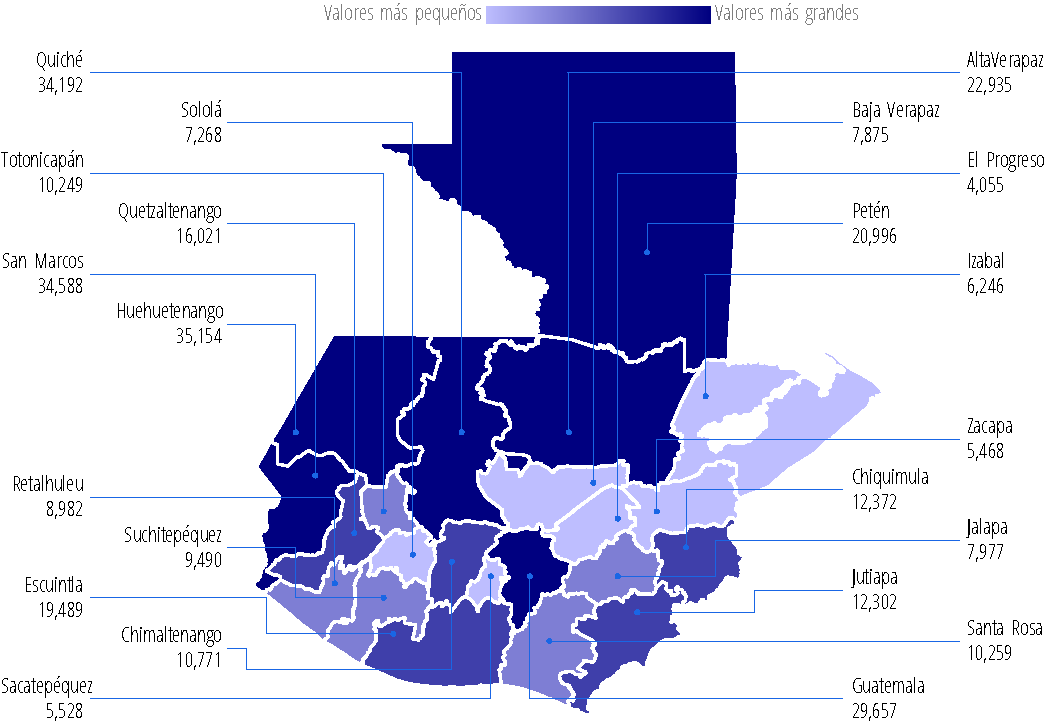
\includegraphics[width=52\cuadri]{graficas/5_14.pdf}}%
{%
	Sigsa} %


%#########################15########################

\cajita{%
	Infecciones Respiratorias Agudas (IRA)}%
{%
	En el período de 2011  a 2015 la menor cantidad de infecciones respiratorias agudas que fueron atendidas por personal médico se registró en 2015, siendo un total de 1,184,756.
}%
{%
	Niños menores de cinco años que recibieron atención médica por infecciones respiratorias agudas} %
{%
	República de Guatemala, serie histórica, número de niños} %
{%
	\begin{tikzpicture}[x=1pt,y=1pt]  \input{graficas/5_15.tex}  \end{tikzpicture}}%
{%
	Sigsa} %

%#########################16########################

\cajita{%
	Infecciones respiratorias agudas según sexo}%
{%
	Al igual que en el caso de la atención por diarreas, la cantidad de casos de IRA atendidos por personal médico es muy similar entre hombres y mujeres. 
}%
{%
	Niños menores de cinco años que recibieron atención médica por infecciones respiratorias agudas, según sexo} %
{%
	República de Guatemala, 2015, número de niños} %
{%
	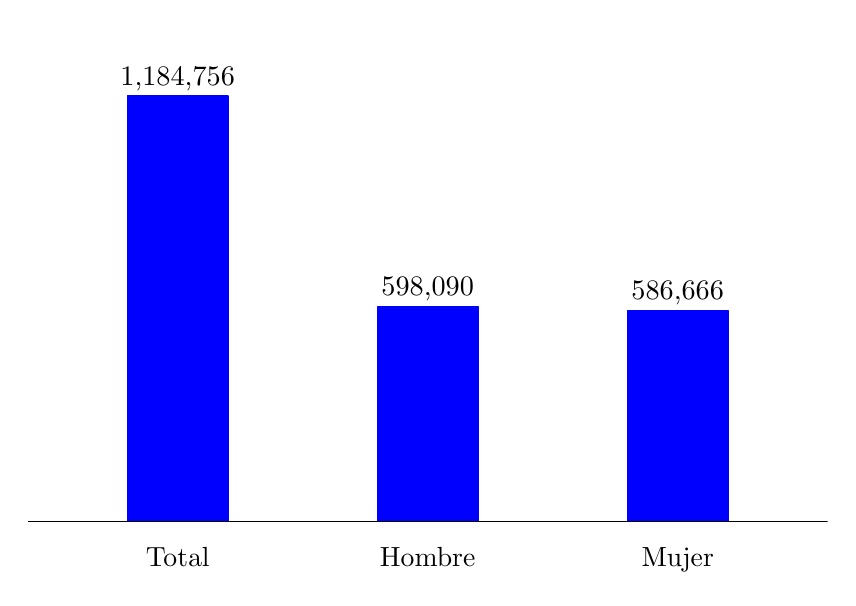
\begin{tikzpicture}[x=1pt,y=1pt]  % Created by tikzDevice version 0.9 on 2016-03-03 05:26:47
% !TEX encoding = UTF-8 Unicode
\definecolor{fillColor}{RGB}{255,255,255}
\path[use as bounding box,fill=fillColor,fill opacity=0.00] (0,0) rectangle (289.08,198.74);
\begin{scope}
\path[clip] (  0.00,  0.00) rectangle (289.08,198.74);

\path[] (  0.00,  0.00) rectangle (289.08,198.74);
\end{scope}
\begin{scope}
\path[clip] (  0.00,  0.00) rectangle (289.08,198.74);

\path[] (  0.00, 12.77) rectangle (289.08,181.67);

\path[] ( 54.20, 12.77) --
	( 54.20,181.67);

\path[] (144.54, 12.77) --
	(144.54,181.67);

\path[] (234.88, 12.77) --
	(234.88,181.67);
\definecolor{drawColor}{RGB}{0,0,255}
\definecolor{fillColor}{RGB}{0,0,255}

\path[draw=drawColor,line width= 0.6pt,line join=round,fill=fillColor] ( 36.13, 20.44) rectangle ( 72.27,173.99);

\path[draw=drawColor,line width= 0.6pt,line join=round,fill=fillColor] (126.47, 20.44) rectangle (162.61, 97.96);

\path[draw=drawColor,line width= 0.6pt,line join=round,fill=fillColor] (216.81, 20.44) rectangle (252.95, 96.48);
\definecolor{drawColor}{RGB}{0,0,0}

\path[draw=drawColor,line width= 0.1pt,line join=round] (  0.00, 20.44) -- (289.08, 20.44);

\node[text=drawColor,anchor=base,inner sep=0pt, outer sep=0pt, scale=  1.02] at ( 54.20,177.96) {1,184,756};

\node[text=drawColor,anchor=base,inner sep=0pt, outer sep=0pt, scale=  1.02] at (144.54,101.93) {598,090};

\node[text=drawColor,anchor=base,inner sep=0pt, outer sep=0pt, scale=  1.02] at (234.88,100.45) {586,666};

\path[] (  0.00, 12.77) rectangle (289.08,181.67);
\end{scope}
\begin{scope}
\path[clip] (  0.00,  0.00) rectangle (289.08,198.74);

\path[] (  0.00, 12.77) --
	(289.08, 12.77);
\end{scope}
\begin{scope}
\path[clip] (  0.00,  0.00) rectangle (289.08,198.74);

\path[] ( 54.20, 10.02) --
	( 54.20, 12.77);

\path[] (144.54, 10.02) --
	(144.54, 12.77);

\path[] (234.88, 10.02) --
	(234.88, 12.77);
\end{scope}
\begin{scope}
\path[clip] (  0.00,  0.00) rectangle (289.08,198.74);
\definecolor{drawColor}{RGB}{0,0,0}

\node[text=drawColor,anchor=base,inner sep=0pt, outer sep=0pt, scale=  1.00] at ( 54.20, 4.00) {Total};

\node[text=drawColor,anchor=base,inner sep=0pt, outer sep=0pt, scale=  1.00] at (144.54, 4.00) {Hombre};

\node[text=drawColor,anchor=base,inner sep=0pt, outer sep=0pt, scale=  1.00] at (234.88, 4.00) {Mujer};
\end{scope}
  \end{tikzpicture}}%
{%
	Sigsa} %

%#########################17########################

\cajota{%
	Casos de IRA por departamento}%
{%
	Los departamentos que registraron mayor cantidad de atención médica de casos de IRA fueron Guatemala (124,186), San Marcos (108,781) y Petén (98,928). 	Los departamentos con la menor cantidad de registros médicos de atención a casos de IRA fueron Zacapa (21,997), Sacatepéquez (20,614) y El Progreso (15,350). 
}%
{%
	Niños menores de cinco años que recibieron atención médica por infecciones respiratorias agudas por departamento} %
{%
	República de Guatemala, departamental, número de niños} %
{%
	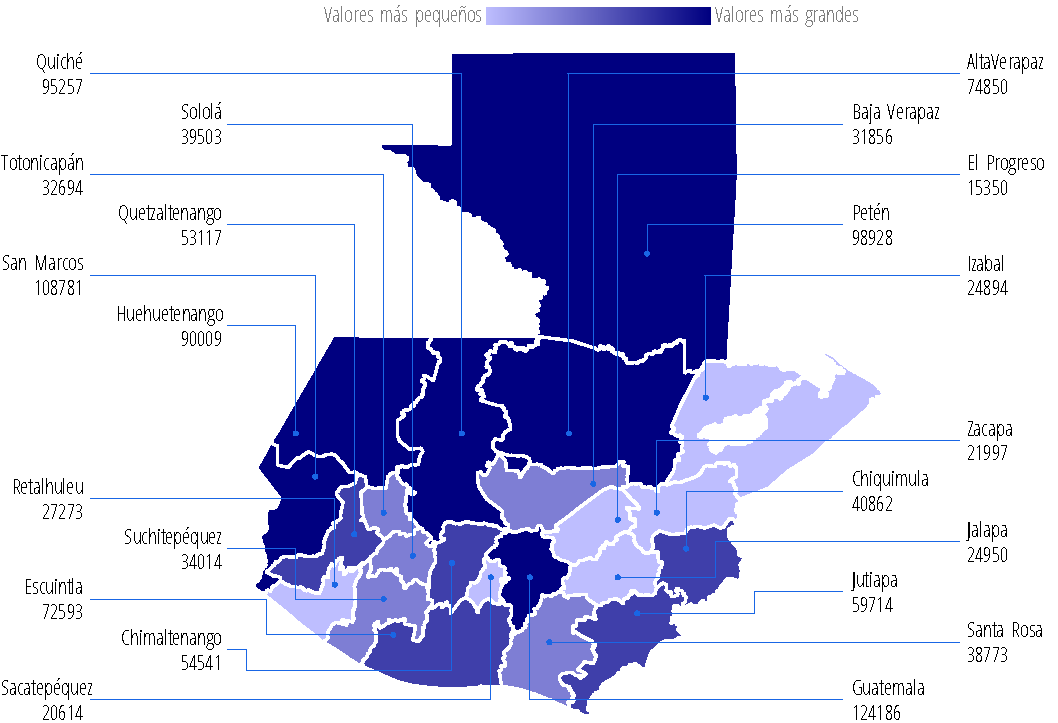
\includegraphics[width=52\cuadri]{graficas/5_17.pdf}}%
{%
	Sigsa} %



%#########################9########################
\stepcounter{section}
\begin{center}
\textbf{\color{color2}\LARGE \thesection} \quad  \textbf{\LARGE Acceso a servicios de Salud} \addcontentsline{toc}{section}{\numberline{\thesection} Acceso a servicios de Salud}
\end{center}
$ \ $ \\[-5cm]
\cajita{%
	Asistencia prenatal}%
{%

En todos los grupos de edad, el porcentaje de mujeres que recibieron atención médica prenatal de un proveedor calificado es al menos del 90\%. 
}%
{%
	Mujeres que recibieron atención prenatal de un proveedor calificado, según grupos de edad} %
{%
	República de Guatemala, 2014, en porcentaje} %
{%
	\begin{tikzpicture}[x=1pt,y=1pt]  \input{graficas/5_09.tex}  \end{tikzpicture}}%
{%
	Ensmi, 2014} %

%#########################10########################

\cajita{%
	Asistencia en el parto}%
{%
	Siete de cada diez mujeres menores de 34 años reciben algún tipo de asistencia médica a la hora del parto, mientras que para mujeres mayores de 34 años este indicador baja a seis de cada diez. 
}%
{%
	Mujeres que recibieron atención a la hora del parto  de un proveedor calificado, según grupos de edad} %
{%
	República de Guatemala, 2014, en porcentaje} %
{%
	\begin{tikzpicture}[x=1pt,y=1pt]  \input{graficas/5_10.tex}  \end{tikzpicture}}%
{%
	Ensmi, 2014} %



%#########################11########################

\cajita{%
	Niños que reciben alguna vacuna o desparasitante}%
{%
	El número de niños que recibe alguna vacuna o desparasitante aumentó en 2015 respecto al 2011. 
	
	El año que presentó mayor cantidad de niños desparasitados o vacunados fue  2012.
}%
{%
	Niños que reciben vacunas o desparasitantes} %
{%
	República de Guatemala, serie histórica, número de niños} %
{%
	\begin{tikzpicture}[x=1pt,y=1pt]  \input{graficas/5_11.tex}  \end{tikzpicture}}%
{%
	Sigsa} %

%#########################7########################

\cajita{%
	Tasa Global de Fecundidad (TGF)}%
{%	
	La Tasa Global de Fecundidad (TGF) ha ido en descenso, ya que en 1995 se ubicó en 5.1, mientras que para el 2014 llegó a 3.1 niños por mujer. 
}%
{%
	Evolución de la tasa global de fecundidad} %
{%
	República de Guatemala, serie histórica, niños por mujer} %
{%
	\begin{tikzpicture}[x=1pt,y=1pt]  \input{graficas/5_07.tex}  \end{tikzpicture}}%
{%
	Ensmi, 2014, 2008, 2002 y 1995} %

%#########################8########################

\cajita{%
	Tasa Global de Fecundidad, por área de residencia}%
{%
	Al analizar la Tasa Global de Fecundidad por área de residencia, se observa que las mujeres en el área urbana tienen menos hijos que las del área rural, esto es 2.5 contra 3.7 niños por mujer respectivamente. 
}%
{%
	Tasa global de fecundidad por área de residencia} %
{%
	República de Guatemala, 2014, niños por mujer} %
{%
	\begin{tikzpicture}[x=1pt,y=1pt]  \input{graficas/5_08.tex}  \end{tikzpicture}}%
{%
	Ensmi, 2014} %




%%%%%%%%%%%%%%%%%%%%%%%%%%%%%%%%%%13%%%%%%%%%%%%%%%%%%%%%%%%
\newpage
\stepcounter{section}
\begin{center}
\textbf{\color{color2}\LARGE \thesection} \quad  \textbf{\LARGE Acceso a servicios básicos} \addcontentsline{toc}{section}{\numberline{\thesection} Acceso a servicios básicos}
\end{center}
$\ $ \\[-2.3cm]
\cajota{%
	Acceso a agua}%
{%
	
	Para el 2011, los departamentos en los cuales más del 50\% de los hogares rurales no contaban con la disponibilidad de agua potable fueron Alta Verapaz y Retalhuleu.}%
{%
	Proporción de hogares del área rural que no poseían acceso a agua potable
} %
{%
	Por departamento, año 2011, en porcentaje} %
{%
	\includegraphics[width=52\cuadri]{graficas/1_14.pdf}}%
{%
	Instituto Nacional de Estadística (INE), Censos Municipales 2008 - 2011.} %




%%%%%%%%%%%%%%%%%%%%%%%%%%%%%%%%%%14%%%%%%%%%%%%%%%%%%%%%%%%

\cajota{%
	Acceso a servicios de saneamiento}%
{%
	Esta necesidad básica clasificada en el acceso a servicios sanitarios, toma las variables de la Encuesta Nacional de Condiciones de Vida (ENCOVI), la cual  recoge datos sobre la disponibilidad de servicios sanitarios y sistemas de eliminación de excretas.
	
	Para el 2011, el 40.4\% de los hogares rurales en Chiquimula no contaba con acceso a servicios de saneamiento, y en Jutiapa, Petén y Jalapa, tres de cada diez hogares del área rural también carecían de este servicio.   }%
{%
	Proporción de hogares del área rural sin acceso a servicios de saneamiento }
{%
	Por departamento, año 2011, en porcentaje} %
{%
	\includegraphics[width=52\cuadri]{graficas/1_15.pdf}}%
{%
	Instituto Nacional de Estadística (INE), Censos Municipales 2008 - 2011. } %


%#########################5########################
\stepcounter{section}
\begin{center}
\textbf{\color{color2}\LARGE \thesection} \quad  \textbf{\LARGE Vivienda} \addcontentsline{toc}{section}{\numberline{\thesection} Vivienda}
\end{center}
$\ $ \\[-5cm]
\cajita{%
	Viviendas y acceso al agua}%
{%
	Para el 2014, el 78.1\% de los hogares contaba con acceso a agua. A pesar de esto se presentan diferencias significativas entre el área rural y el área urbana, teniendo menor acceso esta última.
}%
{%
	Viviendas que tienen acceso a agua, según área de residencia} %
{%
	República de Guatemala, 2014, en porcentaje} %
{%
	\begin{tikzpicture}[x=1pt,y=1pt]  \input{graficas/5_05.tex}  \end{tikzpicture}}%
{%
	Encovi, 2014} %
	

%#########################6########################

\cajita{%
	Viviendas y acceso a drenajes}%
{%
	
	Para el 2014 en la República de Guatemala, el acceso a drenajes no alcanzaba el 50\%. Además, en el área rural apenas el 11.6\% cuenta con drenajes. 
	
}%
{%
	Viviendas que tienen acceso a drenajes según, área	 de residencia} %
{%
	República de Guatemala, 2014, en porcentaje} %
{%
	\begin{tikzpicture}[x=1pt,y=1pt]  \input{graficas/5_06.tex}  \end{tikzpicture}}%
{%
	Encovi, 2014} %



%#########################1########################

 \cajita{%
Viviendas formales }%
{%
	En la República, el 91.4\% de los hogares que no son pobres tiene una vivienda formal, mientras que cerca del 20\%  de los hogares que está en pobreza extrema no cuenta con una vivienda formal.  
 }%
{%
 Hogares con viviendas formales, según tipo de pobreza} %
{%
 República de Guatemala, 2014, en porcentaje} %
{%
 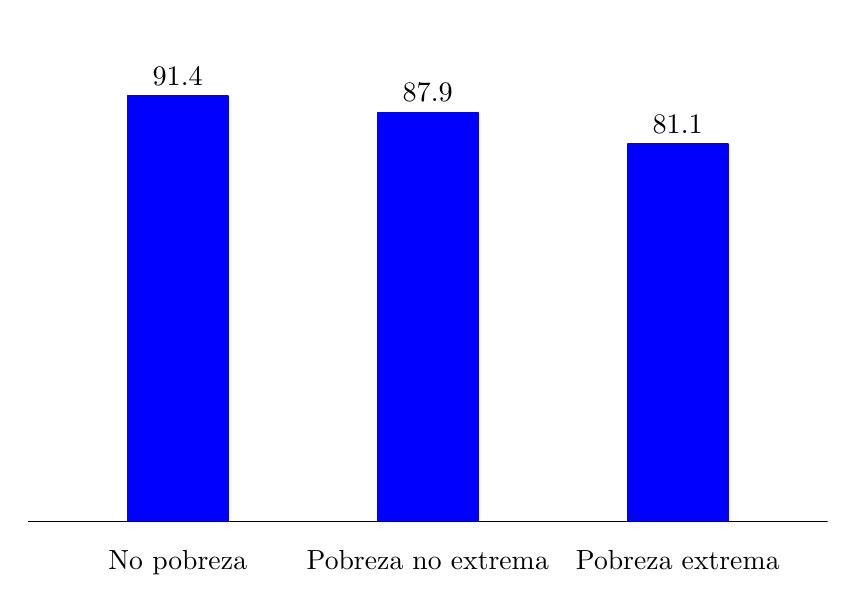
\begin{tikzpicture}[x=1pt,y=1pt]  % Created by tikzDevice version 0.9 on 2016-03-14 17:55:53
% !TEX encoding = UTF-8 Unicode
\definecolor{fillColor}{RGB}{255,255,255}
\path[use as bounding box,fill=fillColor,fill opacity=0.00] (0,0) rectangle (289.08,198.74);
\begin{scope}
\path[clip] (  0.00,  0.00) rectangle (289.08,198.74);

\path[] (  0.00,  0.00) rectangle (289.08,198.74);
\end{scope}
\begin{scope}
\path[clip] (  0.00,  0.00) rectangle (289.08,198.74);

\path[] (  0.00, 12.77) rectangle (289.08,181.67);

\path[] ( 54.20, 12.77) --
	( 54.20,181.67);

\path[] (144.54, 12.77) --
	(144.54,181.67);

\path[] (234.88, 12.77) --
	(234.88,181.67);
\definecolor{drawColor}{RGB}{0,0,255}
\definecolor{fillColor}{RGB}{0,0,255}

\path[draw=drawColor,line width= 0.6pt,line join=round,fill=fillColor] ( 36.13, 20.44) rectangle ( 72.27,173.99);

\path[draw=drawColor,line width= 0.6pt,line join=round,fill=fillColor] (126.47, 20.44) rectangle (162.61,168.11);

\path[draw=drawColor,line width= 0.6pt,line join=round,fill=fillColor] (216.81, 20.44) rectangle (252.95,156.69);
\definecolor{drawColor}{RGB}{0,0,0}

\path[draw=drawColor,line width= 0.1pt,line join=round] (  0.00, 20.44) -- (289.08, 20.44);

\node[text=drawColor,anchor=base,inner sep=0pt, outer sep=0pt, scale=  1.02] at ( 54.20,177.96) {91.4};

\node[text=drawColor,anchor=base,inner sep=0pt, outer sep=0pt, scale=  1.02] at (144.54,172.08) {87.9};

\node[text=drawColor,anchor=base,inner sep=0pt, outer sep=0pt, scale=  1.02] at (234.88,160.66) {81.1};

\path[] (  0.00, 12.77) rectangle (289.08,181.67);
\end{scope}
\begin{scope}
\path[clip] (  0.00,  0.00) rectangle (289.08,198.74);

\path[] (  0.00, 12.77) --
	(289.08, 12.77);
\end{scope}
\begin{scope}
\path[clip] (  0.00,  0.00) rectangle (289.08,198.74);

\path[] ( 54.20, 10.02) --
	( 54.20, 12.77);

\path[] (144.54, 10.02) --
	(144.54, 12.77);

\path[] (234.88, 10.02) --
	(234.88, 12.77);
\end{scope}
\begin{scope}
\path[clip] (  0.00,  0.00) rectangle (289.08,198.74);
\definecolor{drawColor}{RGB}{0,0,0}

\node[text=drawColor,anchor=base,inner sep=0pt, outer sep=0pt, scale=  1.00] at ( 54.20, 3.00) {No pobreza};

\node[text=drawColor,anchor=base,inner sep=0pt, outer sep=0pt, scale=  1.00] at (144.54, 3.00) {Pobreza no extrema};

\node[text=drawColor,anchor=base,inner sep=0pt, outer sep=0pt, scale=  1.00] at (234.88, 3.00) {Pobreza extrema};
\end{scope}
  \end{tikzpicture}}%
{%
 Encovi, 2014} %



%%%%%%%%%%%%%%%%%%%%%%%%%%%%%%%%%%12%%%%%%%%%%%%%%%%%%%%%%%%

\cajota{%
	Hogares que viven en hacinamiento en los departamentos}%
{% 
	El hacinamiento toma las variables de la Encuesta Nacional de Condiciones de Vida (ENCOVI), las cuales  recogen información sobre el número de personas en el hogar y el número de cuartos de la vivienda. 	Los departamentos con mayor porcentaje de hogares en el área rural que vivían en hacinamiento en el 2011 fueron: Alta Verapaz (64.8\%), Quiché (59.9\%), Huehuetenango (54.6\%), San Marcos (54.6\%), Suchitepéquez (52.7\%), Izabal (52.5\%), Petén (51.4\%), y Jalapa (51.4\%). }%
{%
	Proporción de hogares del área rural que vive en hacinamiento
} %
{%
	Por departamento, año 2011, en porcentaje} %
{%
	\includegraphics[width=52\cuadri]{graficas/1_13.pdf}}%
{%
 Encovi, 2014} %


%#########################2########################

\cajita{%
	Viviendas con pared de block }%
{%
	Para el 2014, apenas el 22\% de los hogares en pobreza extrema tenía una vivienda con pared de block, mientras que en los hogares que  no son pobres este indicador se ubicaba en 75.7\%. 
}%
{%
	Viviendas con pared de block, según tipo de pobreza} %
{%
	República de Guatemala, 2014, en porcentaje} %
{%
	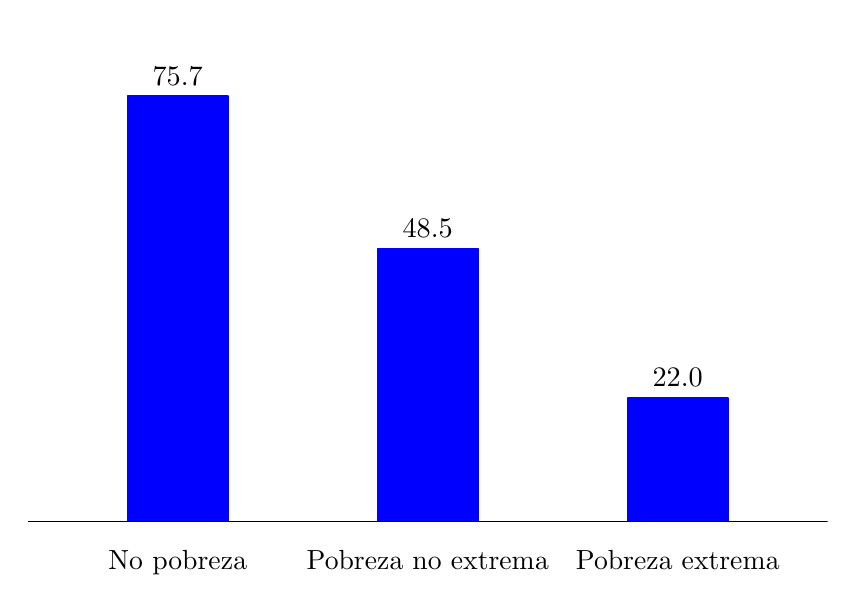
\begin{tikzpicture}[x=1pt,y=1pt]  % Created by tikzDevice version 0.9 on 2016-03-14 17:57:53
% !TEX encoding = UTF-8 Unicode
\definecolor{fillColor}{RGB}{255,255,255}
\path[use as bounding box,fill=fillColor,fill opacity=0.00] (0,0) rectangle (289.08,198.74);
\begin{scope}
\path[clip] (  0.00,  0.00) rectangle (289.08,198.74);

\path[] (  0.00,  0.00) rectangle (289.08,198.74);
\end{scope}
\begin{scope}
\path[clip] (  0.00,  0.00) rectangle (289.08,198.74);

\path[] (  0.00, 12.77) rectangle (289.08,181.67);

\path[] ( 54.20, 12.77) --
	( 54.20,181.67);

\path[] (144.54, 12.77) --
	(144.54,181.67);

\path[] (234.88, 12.77) --
	(234.88,181.67);
\definecolor{drawColor}{RGB}{0,0,255}
\definecolor{fillColor}{RGB}{0,0,255}

\path[draw=drawColor,line width= 0.6pt,line join=round,fill=fillColor] ( 36.13, 20.44) rectangle ( 72.27,173.99);

\path[draw=drawColor,line width= 0.6pt,line join=round,fill=fillColor] (126.47, 20.44) rectangle (162.61,118.90);

\path[draw=drawColor,line width= 0.6pt,line join=round,fill=fillColor] (216.81, 20.44) rectangle (252.95, 65.03);
\definecolor{drawColor}{RGB}{0,0,0}

\path[draw=drawColor,line width= 0.1pt,line join=round] (  0.00, 20.44) -- (289.08, 20.44);

\node[text=drawColor,anchor=base,inner sep=0pt, outer sep=0pt, scale=  1.02] at ( 54.20,177.96) {75.7};

\node[text=drawColor,anchor=base,inner sep=0pt, outer sep=0pt, scale=  1.02] at (144.54,122.87) {48.5};

\node[text=drawColor,anchor=base,inner sep=0pt, outer sep=0pt, scale=  1.02] at (234.88, 69.00) {22.0};

\path[] (  0.00, 12.77) rectangle (289.08,181.67);
\end{scope}
\begin{scope}
\path[clip] (  0.00,  0.00) rectangle (289.08,198.74);

\path[] (  0.00, 12.77) --
	(289.08, 12.77);
\end{scope}
\begin{scope}
\path[clip] (  0.00,  0.00) rectangle (289.08,198.74);

\path[] ( 54.20, 10.02) --
	( 54.20, 12.77);

\path[] (144.54, 10.02) --
	(144.54, 12.77);

\path[] (234.88, 10.02) --
	(234.88, 12.77);
\end{scope}
\begin{scope}
\path[clip] (  0.00,  0.00) rectangle (289.08,198.74);
\definecolor{drawColor}{RGB}{0,0,0}

\node[text=drawColor,anchor=base,inner sep=0pt, outer sep=0pt, scale=  1.00] at ( 54.20, 3.00) {No pobreza};

\node[text=drawColor,anchor=base,inner sep=0pt, outer sep=0pt, scale=  1.00] at (144.54, 3.00) {Pobreza no extrema};

\node[text=drawColor,anchor=base,inner sep=0pt, outer sep=0pt, scale=  1.00] at (234.88, 3.00) {Pobreza extrema};
\end{scope}
  \end{tikzpicture}}%
{%
	Encovi, 2014} %

%#########################3########################

\cajita{%
	Viviendas con techo de lámina }%
{%
Los hogares que no son pobres utilizan en menor medida la lámina para la construcción del techo, con una diferencia cercana a los 25 puntos respecto a los hogares en pobreza extrema. 
	}%
{%
	Viviendas con techo de lámina,  según tipo de pobreza} %
{%
	República de Guatemala, 2014, en porcentaje} %
{%
	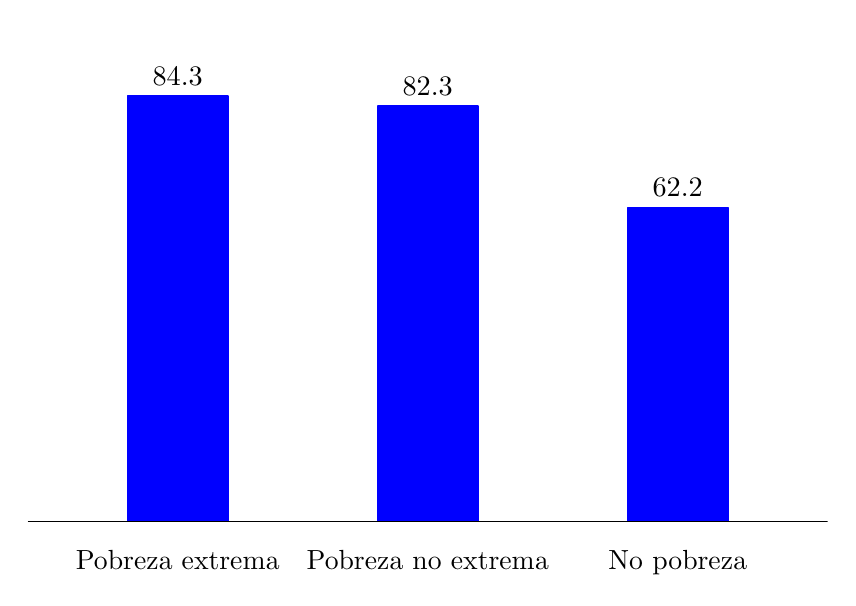
\begin{tikzpicture}[x=1pt,y=1pt]  % Created by tikzDevice version 0.9 on 2016-03-14 17:57:53
% !TEX encoding = UTF-8 Unicode
\definecolor{fillColor}{RGB}{255,255,255}
\path[use as bounding box,fill=fillColor,fill opacity=0.00] (0,0) rectangle (289.08,198.74);
\begin{scope}
\path[clip] (  0.00,  0.00) rectangle (289.08,198.74);

\path[] (  0.00,  0.00) rectangle (289.08,198.74);
\end{scope}
\begin{scope}
\path[clip] (  0.00,  0.00) rectangle (289.08,198.74);

\path[] (  0.00, 12.77) rectangle (289.08,181.67);

\path[] ( 54.20, 12.77) --
	( 54.20,181.67);

\path[] (144.54, 12.77) --
	(144.54,181.67);

\path[] (234.88, 12.77) --
	(234.88,181.67);
\definecolor{drawColor}{RGB}{0,0,255}
\definecolor{fillColor}{RGB}{0,0,255}

\path[draw=drawColor,line width= 0.6pt,line join=round,fill=fillColor] ( 36.13, 20.44) rectangle ( 72.27,173.99);

\path[draw=drawColor,line width= 0.6pt,line join=round,fill=fillColor] (126.47, 20.44) rectangle (162.61,170.40);

\path[draw=drawColor,line width= 0.6pt,line join=round,fill=fillColor] (216.81, 20.44) rectangle (252.95,133.74);
\definecolor{drawColor}{RGB}{0,0,0}

\path[draw=drawColor,line width= 0.1pt,line join=round] (  0.00, 20.44) -- (289.08, 20.44);

\node[text=drawColor,anchor=base,inner sep=0pt, outer sep=0pt, scale=  1.02] at ( 54.20,177.96) {84.3};

\node[text=drawColor,anchor=base,inner sep=0pt, outer sep=0pt, scale=  1.02] at (144.54,174.38) {82.3};

\node[text=drawColor,anchor=base,inner sep=0pt, outer sep=0pt, scale=  1.02] at (234.88,137.71) {62.2};

\path[] (  0.00, 12.77) rectangle (289.08,181.67);
\end{scope}
\begin{scope}
\path[clip] (  0.00,  0.00) rectangle (289.08,198.74);

\path[] (  0.00, 12.77) --
	(289.08, 12.77);
\end{scope}
\begin{scope}
\path[clip] (  0.00,  0.00) rectangle (289.08,198.74);

\path[] ( 54.20, 10.02) --
	( 54.20, 12.77);

\path[] (144.54, 10.02) --
	(144.54, 12.77);

\path[] (234.88, 10.02) --
	(234.88, 12.77);
\end{scope}
\begin{scope}
\path[clip] (  0.00,  0.00) rectangle (289.08,198.74);
\definecolor{drawColor}{RGB}{0,0,0}

\node[text=drawColor,anchor=base,inner sep=0pt, outer sep=0pt, scale=  1.00] at ( 54.20, 3.00) {Pobreza extrema};

\node[text=drawColor,anchor=base,inner sep=0pt, outer sep=0pt, scale=  1.00] at (144.54, 3.00) {Pobreza no extrema};

\node[text=drawColor,anchor=base,inner sep=0pt, outer sep=0pt, scale=  1.00] at (234.88, 3.00) {No pobreza};
\end{scope}
  \end{tikzpicture}}%
{%
	Encovi, 2014} %

%#########################4########################

\cajita{%
	Viviendas y material del piso}%
{%
	Los hogares en   pobreza extrema son los que presentan una menor proporción en el uso de torta de cemento (25.3\% contra un 67\%). Para los hogares que no son pobres predomina el uso de torta de cemento, ya que el 40.2\% de los hogares lo usa, contra un 10.4\% que usa piso de tierra. 
}%
{%
	Viviendas según material del piso y tipo de pobreza} %
{%
	República de Guatemala, 2014, en porcentaje} %
{%
	\begin{tikzpicture}[x=1pt,y=1pt]  % Created by tikzDevice version 0.9 on 2016-03-03 05:25:52
% !TEX encoding = UTF-8 Unicode
\definecolor{fillColor}{RGB}{255,255,255}
\path[use as bounding box,fill=fillColor,fill opacity=0.00] (0,0) rectangle (289.08,198.74);
\begin{scope}
\path[clip] (  0.00,  0.00) rectangle (289.08,198.74);

\path[] (  0.00,  0.00) rectangle (289.08,198.74);
\end{scope}
\begin{scope}
\path[clip] (  0.00,  0.00) rectangle (289.08,198.74);

\path[] (  0.00, 18.46) rectangle (289.08,166.57);

\path[] ( 54.20, 18.46) --
	( 54.20,166.57);

\path[] (144.54, 18.46) --
	(144.54,166.57);

\path[] (234.88, 18.46) --
	(234.88,166.57);
\definecolor{drawColor}{RGB}{0,0,255}
\definecolor{fillColor}{RGB}{0,0,255}

\path[draw=drawColor,line width= 0.6pt,line join=round,fill=fillColor] ( 15.81, 18.46) rectangle ( 51.94, 74.33);
\definecolor{drawColor}{RGB}{157,187,255}
\definecolor{fillColor}{RGB}{157,187,255}

\path[draw=drawColor,line width= 0.6pt,line join=round,fill=fillColor] ( 56.46, 18.46) rectangle ( 92.60,166.57);
\definecolor{drawColor}{RGB}{0,0,255}
\definecolor{fillColor}{RGB}{0,0,255}

\path[draw=drawColor,line width= 0.6pt,line join=round,fill=fillColor] (106.15, 18.46) rectangle (142.28,120.72);
\definecolor{drawColor}{RGB}{157,187,255}
\definecolor{fillColor}{RGB}{157,187,255}

\path[draw=drawColor,line width= 0.6pt,line join=round,fill=fillColor] (146.80, 18.46) rectangle (182.93, 95.86);
\definecolor{drawColor}{RGB}{0,0,255}
\definecolor{fillColor}{RGB}{0,0,255}

\path[draw=drawColor,line width= 0.6pt,line join=round,fill=fillColor] (196.48, 18.46) rectangle (232.62,107.27);
\definecolor{drawColor}{RGB}{157,187,255}
\definecolor{fillColor}{RGB}{157,187,255}

\path[draw=drawColor,line width= 0.6pt,line join=round,fill=fillColor] (237.14, 18.46) rectangle (273.27, 41.36);
\definecolor{drawColor}{RGB}{0,0,0}

\path[draw=drawColor,line width= 0.6pt,line join=round] (  0.00, 18.46) -- (289.08, 18.46);

\node[text=drawColor,rotate= 90.00,anchor=base west,inner sep=0pt, outer sep=0pt, scale=  0.83] at ( 37.11, 76.88) {25.3};

\node[text=drawColor,rotate= 90.00,anchor=base west,inner sep=0pt, outer sep=0pt, scale=  0.83] at ( 77.76,169.12) {67.0};

\node[text=drawColor,rotate= 90.00,anchor=base west,inner sep=0pt, outer sep=0pt, scale=  0.83] at (127.45,123.26) {46.3};

\node[text=drawColor,rotate= 90.00,anchor=base west,inner sep=0pt, outer sep=0pt, scale=  0.83] at (168.10, 98.40) {35.0};

\node[text=drawColor,rotate= 90.00,anchor=base west,inner sep=0pt, outer sep=0pt, scale=  0.83] at (217.79,109.81) {40.2};

\node[text=drawColor,rotate= 90.00,anchor=base west,inner sep=0pt, outer sep=0pt, scale=  0.83] at (258.44, 43.91) {10.4};

\path[] (  0.00, 18.46) rectangle (289.08,166.57);
\end{scope}
\begin{scope}
\path[clip] (  0.00,  0.00) rectangle (289.08,198.74);

\path[] (  0.00, 18.46) --
	(289.08, 18.46);
\end{scope}
\begin{scope}
\path[clip] (  0.00,  0.00) rectangle (289.08,198.74);

\path[] ( 54.20, 15.71) --
	( 54.20, 18.46);

\path[] (144.54, 15.71) --
	(144.54, 18.46);

\path[] (234.88, 15.71) --
	(234.88, 18.46);
\end{scope}
\begin{scope}
\path[clip] (  0.00,  0.00) rectangle (289.08,198.74);
\definecolor{drawColor}{RGB}{0,0,0}

\node[text=drawColor,anchor=base,inner sep=0pt, outer sep=0pt, scale=  1.00] at ( 54.20,  5.69) {Pobreza extrema};

\node[text=drawColor,anchor=base,inner sep=0pt, outer sep=0pt, scale=  1.00] at (144.54,  5.69) {Pobreza no extrema};

\node[text=drawColor,anchor=base,inner sep=0pt, outer sep=0pt, scale=  1.00] at (234.88,  5.69) {No pobreza};
\end{scope}
\begin{scope}
\path[clip] (  0.00,  0.00) rectangle (289.08,198.74);
\coordinate (apoyo) at (41.26,191.13);
\coordinate (longitudFicticia) at (7.11,7.61);
\coordinate (longitud) at (7.11,7.11);
\coordinate (desX) at (157.45,0);
\coordinate (desY) at (0,0.25);
\definecolor[named]{ct1}{HTML}{
0000FF
}
\definecolor[named]{ct2}{HTML}{
9DBBFF
}
\definecolor[named]{ctb1}{HTML}{
0000FF
}
\definecolor[named]{ctb2}{HTML}{
9DBBFF
}
\path [fill=none] (apoyo) rectangle ($(apoyo)+(longitudFicticia)$)
node [xshift=0.3cm,inner sep=0pt, outer sep=0pt,midway,right,scale = 0.9]{Torta de cemento};
\draw [color = ctb1,fill=ct1] ( $(apoyo)  + (desY) $) rectangle ($(apoyo)+ (desY) +(longitud)$);
\path [fill=none] ($(apoyo)+(desX)$) rectangle ($(apoyo)+(desX)+(longitudFicticia)$)
node [xshift=0.3cm,inner sep=0pt, outer sep=0pt,midway,right,scale = 0.9]{Tierra};
\draw [color = ctb2 ,fill=ct2] ( $(apoyo)  + (desY) + (desX) $) rectangle ($(apoyo)+ (desY)+ (desX) +(longitud)$);
\end{scope}
  \end{tikzpicture}}%
{%
	Encovi, 2014} %

